\chapter{Discussion and future work}
\label{toc:discussion}
This thesis presented an introduction to Bayesian machine learning based on statistical learning theory.
A machine learning problem was characterized as an under-specified computational problem that requires additional subjective assumptions to solve.
In a regression problem, finitely many observations are used to select an infinite-dimensional object, a function that explains them well.
Bayesian generative models are a tool to formalize complex assumptions about these functions and Bayesian inference offers a principled method for model selection, combining prior assumptions with the ideas of empirical risk minimization.
\todo{Rework after thesis outline}
The topic of this thesis is to explore how general function approximators such as Gaussian processes can be embedded in hierarchical generative models to combine the benefits of expressive prior knowledge with the ability to gain new insights from data.

\Cref{toc:data_association} introduced a Bayesian approach to the data association problem, where we consider a data set that has been generated by a mixture of processes and we are interested in factorizing the data into these components.
A fully Bayesian model can produce such a factorization and yield models that explain observations well.
However, since empirical risk minimization only evaluates the predictive distribution of a model and does not consider its internal structure, hierarchical models can introduce qualitative ambiguities:
As long as they result in the same predictive distribution and are equally plausible under a structural prior, Bayesian model selection cannot distinguish between more and less interpretable or desirable solutions.
In the general data association problem, formalizing desirable solutions via specific dependency structures between is a hard problem from both the modeling and inference points of view.

\Cref{toc:alignment} considered how to achieve sich a formalization in the more specific problem domain of time-series alignment.
The chapter viewed the power production of different wind turbines in a wind farm as a multi-modal time-series with shared latent information, the wind fronts interacting with the turbines.
Hierarchical structure is introduced by the alignment problem of how wind fronts move through the system.
By formulating a strong prior on the dependence between modes through a multi-output GP and encoding knowledge about the underlying physical system, ambiguities can be avoided and rich structure can be learned.
A strong prior simplifies inference but also limits what can be learned from data based on subjective notions of what makes a model good or correct.

\cref{toc:interpretable_rl} explored how this subjectiveness can be incorporated into the model itself.
Taking the wet-chicken reinforcement learning problem as an example, a model is formulated based on high-level prior knowledge about the system dynamics decomposing the inference task into interpretable components.
The correctness of the model can be evaluated through experts inspecting the interpretable components and the downstream performance in the reinforcement learning task.
We showed that while misspecified models yielded similar predictive distributions to semantically correct models, a well-specified model can solve the posed task significantly better.

In this chapter, we explore how taking downstream tasks can affect modeling decisions and discuss challenges during inference.
A Bayesian posterior of a hierarchical generative process with general function approximators can be very complex and the fewer constraints are put on it, the more heterogeneous it can be.
The inference schemes for hierarchical Gaussian process models introduced in \cref{toc:dgp} rely on variational independence assumptions between components to achieve computational tractability.
In \cref{toc:alignment}, we saw that these inference schemes can struggle when posteriors become complex.
In \cref{toc:discussion:composition}, we present an intuitive argument for why inference schemes based on factorizations between layers cannot represent heterogeneous posteriors.
Empirical risk minimization through high marginal likelihoods in Bayesian model selection is not always enough to identify semantically correct hierarchical models as it does not consider internal structure.
Undesired explanations of the data can be removed from the posterior by formulating priors with strong constraints as discussed in \cref{toc:alignment}.
However, this approach requires extensive prior knowledge and limits what can be learned from data.
In \cref{toc:interpretable_rl}, model selection was realized through policy search in a reinforcement learning problem.
In \cref{toc:discussion:bo,toc:discussion:mountaincar} we explore this idea further and consider how tasks can be included in the inference problem directly.
In \cref{toc:discussion:future_work} we discuss possible further directions of research.


\section{Compositional uncertainty in hierarchical models}
\label{toc:discussion:composition}
\begin{figure}[t]
    \centering
    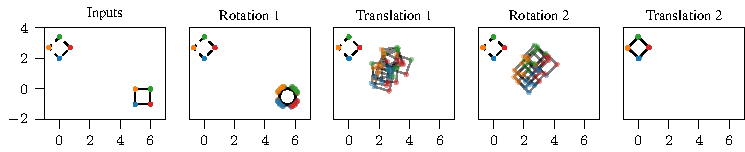
\includegraphics[width=\textwidth]{rotated_squares_example}
    \caption{
        \label{fig:composition:rotated_squares_example}
        Compositional model (toy example): the transformation of the solid rectangle onto the dashed one is decomposed as $T_2 \circ R_2 \circ T_1 \circ R_1$ where $R_i$ and $T_i$ are rotations and translations.
        Different sampled realizations of these transformations are overlaid, showing the \emph{compositional uncertainty}.
        Approximating $R_i$ and $T_i$ as independent transformations does not allow us to capture such uncertainty, collapsing to a single realisation of the composition.
    }
\end{figure}
\begin{figure}[t]
    \centering
    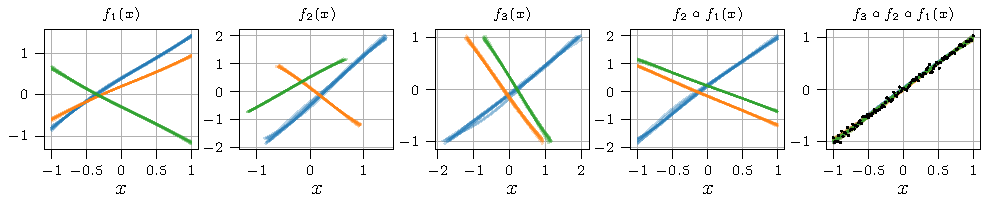
\includegraphics[width=\textwidth]{factorized_dgp_identity}
    \caption{
        \label{fig:composition:identity_factorised}
        Example fits of a three-layer DGP \emph{with factorised inducing points} to a data set shown in the rightmost panel (black dots).
        Different panels show the computations performed by each of the three layers and their compositions.
        Different colours correspond to three models fitted to the same data with different random initialisations.
        For each initialisation, ten samples (of the same colour) from the fitted model are shown on top of each other.
    }
\end{figure}
Hierarchical learning studies functions represented as compositions of other functions, $f = f_L \circ \ldots \circ f_1$.
Such models provide a natural way to model data generated by a hierarchical process, as each $f_\ell$ represents a certain part of the hierarchy, and the prior assumptions on $\{f_\ell\}_{\ell=1}^{L}$ reflect the corresponding prior assumptions about the data generating process.
DGPs~\parencite{Damianou:2013}, which are compositions of GPs, allow us to impose explicit prior assumptions on $\{f_\ell\}$ by choosing the corresponding kernels.
By computing the posterior distributions of $\{f_\ell\}$, we can uncover the structure of the data and explicitly estimate the uncertainties due to each function (or layer) in the composition.
Since different compositions can fit the data equally well (see an illustration in \cref{fig:rotated_squares_example}), DGPs are inherently unidentifiable, and this lack of identifiability should be captured by an adequate Bayesian posterior, allowing us to quantify uncertainties pertaining to each $f_\ell$.
We refer to this uncertainty as \emph{compositional uncertainty}. This uncertainty can be thought of as the epistemic uncertainty~\parencite{Gal:2016} describing how the layers of the hierarchy jointly compose the observed data.

While the DGP posterior captures compositional uncertainty, exact Bayesian inference in DGPs is intractable~\parencite{Damianou:2013}.
In this work we show that the typically used approximate inference schemes \parencite[e.g.][]{Salimbeni:2017} impose strong simplifying assumptions, making intermediate DGP layers collapse to deterministic transformations.
In cases where the data has high observational noise, the noise is explained by introducing an uncertainty in one or multiple layers of the composition.
We focus on the case where the data is noiseless, thus the uncertainty in each of the layers arises only due to the ambiguity in the compositional structure.
This corresponds to representing a DGP as a single-layer GP with a transformed kernel~\parencite{Dunlop:2018}, similar to GPs with kernels parametrised by a deterministic function (e.g.\ a neural network).
Such behaviour might not be a problem in practice if the goal is to design a model that only provides a high marginal likelihood of the data, however, it does not make full use of the capacity of DGP as it fails to describe the uncertainty that stems from the potential decomposition in the hierarchy.
Distributions over compositions, and the resulting compositional uncertainty, are important for applications, for example for temporal alignment of time series data~\parencite{Kaiser:2018, Kazlauskaite:2019}, in reinforcement learning~\parencite{Jin:2017} as well as for building more interpretable models where each layer in the hierarchy expresses a meaningful functional prior~\parencite{Sun:2019}.

We address the issue of collapsing compositional uncertainty by proposing variational distributions and corresponding inference methods that explicitly model the dependencies between the layers, resulting in variational posteriors that capture compositional uncertainty.
We highlight the limitations of existing approaches and lay the ground for future work in uncertainty quantification in DGPs.

If a DGP $f_L \circ \ldots \circ f_1$ maps fixed inputs $X$ to fixed outputs $Y$, the functions $\{f_\ell\}$ must be dependent, because every realisation of this composition must map the \emph{same} $X$ to the \emph{same} $Y$.
This is illustrated in~\cref{fig:toy_example}, which shows a composition of three layers, each of which could either be $f_\ell(x) = x$ or $f_\ell(x) = -x$.
Depending on the choices of $f_1$ and $f_2$, the input is mapped by $f_2 \circ f_1$ to one of the two realisations of $F_2$ (as shown by the colour code in the corresponding panel), and $f_3$ must be chosen in such a way that $F_2$ is mapped to $Y$.
Therefore, in this example, $f_3$ depends on the choice of $f_1$ and $f_2$.
However, if $\{f_\ell\}$ were independent, then the only way to ensure that every realisation of the composition fits the data would be for each layer to implement a deterministic transformation (i.e.\ either $f_\ell(x) = x$ or $f_\ell(x) = -x$ such that there are zero or two instances of $f_\ell(x) = -x$).
Another illustration of this idea is provided in~\cref{fig:rotated_squares_example}, in which movement of a square is represented as a composition of correlated rotations and translations, allowing us to see a variety of possible movements.
However, a model with independent transformations would converge to a single possible sequence of rotations and translations.

The same intuition holds for general DGPs. Analogously to choosing either $x$ or $-x$ in~\cref{fig:toy_example}, inducing locations $Z_\ell$ and points $U_\ell$ define the transformation implemented by the corresponding layer through the predictive posterior $p(F_\ell \mid F_{\ell-1}, U_\ell, Z_{\ell-1})$. Following a similar argument, the DGP layers collapse to deterministic transformations to ensure good data fits unless they are dependent to allow multiple different compositions to fit the data.


\section{Bayesian Optimization}
\label{toc:discussion:bo}
\begin{figure}[t]
    \centering
    \raisebox{-0.5\height}{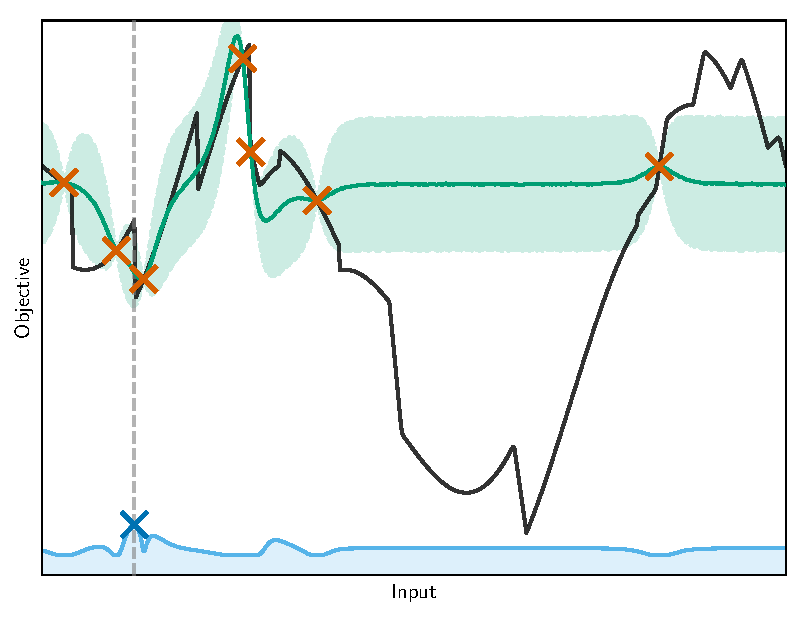
\includegraphics[trim=15 15 0 0, clip, width=0.25\textwidth]{robust_bo_erik/illustrative_figure/gp.pdf}}
    \raisebox{-0.5\height}{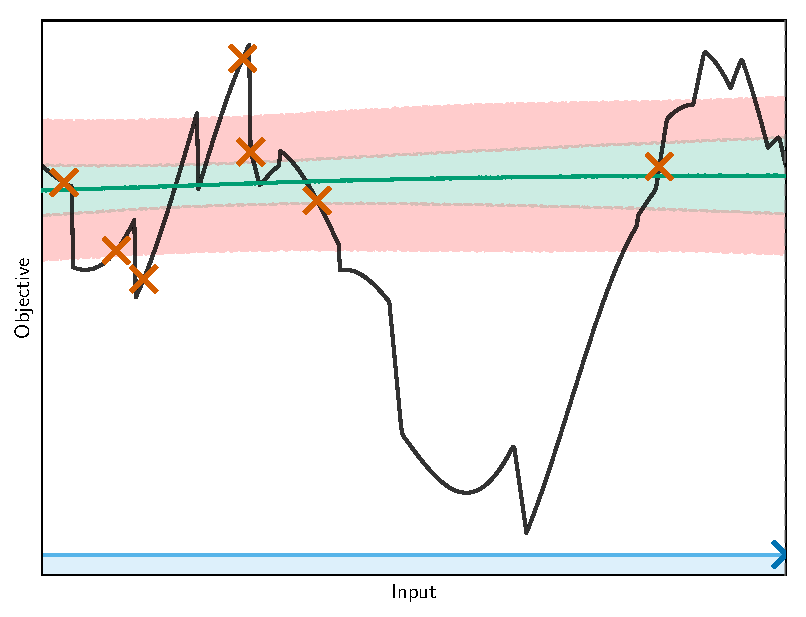
\includegraphics[trim=15 15 0 0, clip, width=0.25\textwidth]{robust_bo_erik/illustrative_figure/homo_gp.pdf}}
    \raisebox{-0.5\height}{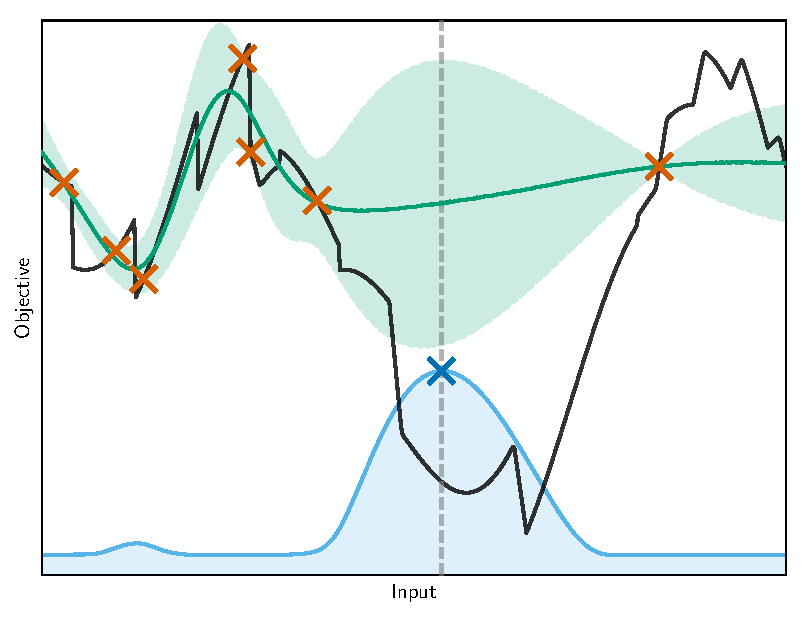
\includegraphics[trim=15 15 0 0, clip, width=0.25\textwidth]{robust_bo_erik/illustrative_figure/modulating_lgp.pdf}}
    \raisebox{-0.45\height}{{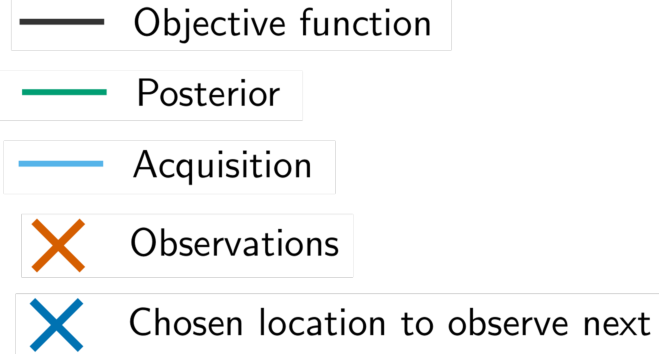
\includegraphics[width=0.20\textwidth]{robust_bo_erik/illustrative_figure/legend_compact.pdf}}}
    \caption{
        \label{fig:bo:posterior}
        As a result, the acquisition function can utilize a confidently discovered global trend to increase the efficiency of the search.
    }
\end{figure}
Bayesian optimization (BO)~\cite{snoek2012practical} is a method for finding the optimum of functions that are unknown and expensive to evaluate.
By fitting a surrogate model to the samples of an unknown objective, the BO procedure iteratively picks the new samples of the objective believed to be the most informative about where the optimum is located.

Model misspecification has significant negative implications for any machine learning tasks.
This is especially true for sequential decision making tasks such as BO, where the model is used not only to locate the optimum based on the collected data but also to decide where to collect data for future decisions.
If the surrogate model is misspecified, it is likely to acquire samples that are less informative about the optimum, which will lead to a less efficient optimization.
Therefore the quality of the surrogate model is essential to achieve both efficient and reliable results.

Many works have been done towards avoiding model misspecification in the surrogate model for BO, such as handling non-stationary objective functions with warpings~\cite{snoek2014input}, tree-structured dependencies in the search space~\cite{jenatton2017bayesian}, and searching the optimum from piecewise comparisons~\cite{gonzalez2017preferential}.
Comparing with the Gaussian process (GP) regression model in the standard BO setting, these methods avoid model misspecification in real-world problems by using more sophisticated surrogate models that are suitable for the corresponding problems.
Bayesian inference with more sophisticated surrogate models will often require additional data to reduce uncertainty and confirm beliefs, because it considers more possibilities.
Importantly the ultimate goal of BO is to find the optimum, not to model the unknown objective as precisely as possible.
In practice, this means that using a surrogate with high complexity might perform worse compared to a simpler class
even if the former contains the true objective function.

Instead of building a complex surrogate model with minimal model misspecification,
we propose an alternative approach which allows trading off accuracy in modeling the objective with efficiency of capturing informative structures from small amounts of data.
For example, we observe that structures such as local oscillations and discontinuities are less important to capture for the purposes of BO.
Such details often require a lot of data to be closely captured in a surrogate model but do not help the search for the optimum,
unless the search reaches the last stage of pinpointing the exact location of the optimum.
To ignore these details, we associate an independent random \emph{input} variable with every evaluation of the unknown function.
As the random variables associated with new evaluations are conditionally independent of the posterior random variables associated with observed data given the function,
this is referred to as \emph{irreducible uncertainty}.
Such variables are similar to the noise variables in regression models, which are used to capture measurement noise and the data variance that cannot be attributed to the input variables.
In contrast to noise variables for noisy outcomes,
where there is irreducible uncertainty about the data, there is now irreducible uncertainty in the model of the function.

We propose to use the surrogate models that are specified over well-behaved approximations of the objectives,
which can be more useful for the search of the optimum (see Figure~\ref{fig:posterior}), augmented with flexible ``noise" distributions to treat the nuisance parameters.
We will demonstrate that, using the same function approximation, a surrogate model with a more flexible nuisance parameter distribution is more robust against challenging structures.
In this paper we focus on noise-free objectives with complicated, oscillatory or discontinuous structures.
In particular, we propose to use a Latent Gaussian process (LGP)~\cite{pfingsten2006nonstationary,wang12_gauss_proces_regres_with_heter,yousefi_unsupervised_2016,bodin_latent_2017} as the surrogate model due to its flexible nuisance parameter distribution and show that it outperforms the surrogate models with less flexible distributions such as GPs with additive likelihoods.
LGP allows us to disentangle the complicated structures a GP surrogate struggles to model while highlighting important structures.

Let $f : X \to R$ be an unknown, noise-free objective function defined on a bounded subset $X \subset R^Q$.
The goal of BO is to solve the global optimization problem of finding
\begin{equation}
    \mat{x}_{\text{min}} = \argmin_{\mat{x} \in X} f(\mat{x}).
\end{equation}
In real world problems,
the objective function is often not a well-behaved function and a suitable model is difficult to specify.
Instead of applying an automated model selection method~\cite{malkomes2018automating},
we propose to model only the essential structure of the objective function that is well-behaved and leave the rest of the function details to be absorbed in a noise distribution.

We consider the family of objective functions $f$ that can be represented as a composition of a well-behaved function and another arbitrary, latent function capturing the challenging details, i.e.
\begin{equation}
    \label{eq:well_behaved}
    f(\mat{x}) := g(\mat{x}, \mat{h}), \quad \mat{h}:=h(\mat{x}),
\end{equation}
where $g$ is a well-behaved function that can be nicely modeled by a surrogate model of choice,
which is a Gaussian process (GP) in this paper,
and the vector-valued function $h(\mat{x})$ encodes the structures which the surrogate model struggles to capture.
In general this composition allows for complicated interactions between $\mat{x}$ and $\mat{h}$, producing complicated realizations of the function
which is observed through data.
A simple, special case of a function composition is additive structure
\footnote{Note that in the additive case, $h(\mat{x})$ must match the output in shape, i.e.~be one-dimensional.},
i.e.\ $f(\mat{x}) = g(\mat{x}) + h(\mat{x})$.
%which has been exploited for BO~\cite{gardner2017discovering, mutny2018efficient}.

Instead of modeling $h(\mat{x})$ as part of the surrogate model,
we propose to \textit{ignore} the structure of the objective function in $h(\mat{x})$ by replacing $h(\mat{x})$ with a random variable $\mat{h}$ per data point.
The random variables $\mat{h}$ for different data points  are independent among each other.
The objective function becomes a function of two variables $g(\mat{x}, \mat{h})$,
in which $\mat{h}$ is a random variable which explain the data variance that cannot be explained by $\mat{x}$.
In this paper, we use a normal distribution for the prior of $\mat{h}$, $\mat{h} \sim \mathcal{N}(0,  \mathbb{I})$.
Note that, although the distribution of $h(\mat{x})$ induced by the data distribution for $\mat{x}$ may not be zero-mean and unit-variance, it is easy to reformulate it as a linear transformation of a normal distribution with zero-mean and unit-variance and the resulting linear transformation can be absorbed into the function $g$.
For further details on the definition, see the supplement.

With the above formulation, a BO method can be developed by constructing a model of the well-behaved function $g$
and a model of $h$.
%Data acquisition decisions can then be made based on a function free from the unwanted complicated structures that $h$ captures.
At each step of the BO optimization, a set of input and output pairs of the objective function has been collected, denoted as $\mat{X} = (\mat{x}_1, \ldots, \mat{x}_N)^\top$ and $\mat{F} = (\mat{f}_1, \ldots, \mat{f}_N)^\top$.
The output $\mat{F}$ denotes the noise-free observations of the objective function.
The Bayesian inference of the model aims at inferring the posterior distribution
\begin{equation}
    \Prob{ \mat{H}, \mat{\theta} \given \mat{X}, \mat{F}}  \propto \Prob{\mat{F} \given \mat{X}, \mat{H}, \mat{\theta} }\Prob{\mat{H}}  \Prob{\mat{\theta}}
\end{equation}
where $\mat{\theta}$ are the hyperparameters of the surrogate model and $\mat{H} = (\mat{h}_1, \ldots, \mat{h}_N)^\top$ is the concatenation of the nuisance parameters associated with the individual data points.
The location of the next evaluation is determined according to an acquisition function,
which uses the predictive distribution $\Prob{\mat{f}_* \given \mat{x}_*,  \mat{X}, \mat{F}}$ of the surrogate model,
\begin{align}
    \label{eq:pred_dist}
    \begin{split}
        \MoveEqLeft\Prob{\mat{f}_* \given \mat{x}_*,  \mat{X}, \mat{F}} =
        \int \Prob{\mat{f}_* \given \mat{x}_*, \mat{h}_*, \mat{X}, \mat{F},\mat{H}, \mat{\theta}}\\
        &\qquad\Prob{\mat{H}, \mat{\theta} \given \mat{X}, \mat{F}} \Prob{\mat{h}_*} \diff{\mat{H}}\diff{\mat{\theta}}\diff{\mat{h}_*},
    \end{split}
\end{align}
where $\mat{x}_*$ is the input of the prediction and $\mat{f}_*$ is the noise-free observation at the location $\mat{x}_*$.
The predictive distribution of the latent variable $\Prob{\mat{h}_*}$ associated with new evaluations is as of the i.i.d.~assumption
equal to the prior.
As such $\Prob{\mat{h}_*}$ contains model uncertainty \emph{irreducible} by the active sampling loop,


\section{Bayesian Reinforcement Learning}
\label{toc:discussion:mountaincar}
\begin{figure}[tp]
    \centering
    \includestandalonewithpath{figures/quantities_of_interest_statistical_learning}
    \caption{
        Statistical Learning
        \label{fig:mountaincar:statistical_learning}
    }
\end{figure}
\begin{table}[tp]
    \caption{
        \label{tab:mountaincar:quantities_of_interest}
    }
    \centering
    \newcolumntype{Y}{>{\centering\arraybackslash}X}
    \begin{tabularx}{.9\textwidth}{cYY}
        \toprule
                                  & Statistical Learning   & Reinforcement Learning \\
        \midrule
        $\Prob*{\mat{z}}$         & Latent Distribution    & True system-dynamics   \\
        $\Sc$                     & Observations           & Batch or Online data   \\
        $\Fc$                     & Functional of Interest & Optimal value          \\
        \midrule
        $F : \Probs{\Zc} \to \Fc$ & Functional Operator    & Bellman principle      \\
        $S : \Probs{\Zc} \to \Sc$ & Sampling Operator      & Exploration            \\
        $A : \Sc \to \Fc$         & Learning Algorithm     & Policy search          \\
        \bottomrule
    \end{tabularx}
\end{table}
\begin{figure}[tp]
    \centering
    \includestandalone{graphical_model_rl_deep_gp}
    \caption{
        \label{fig:mountaincar:graphical_model}
        Deep GP RL graphical model.
    }
\end{figure}
At the core of our model is the attempt to formulate the search for a good RL policy in a Bayesian manner.
This means that instead of maintaining or optimizing one candidate policy which gets optimized until some stopping criterion is reached, we want to maintain a Bayesian belief about the optimal policy (or rather one of them).
Intuitively, we want to start off with a very uninformed policy which, given any state, can generate any action.
The inference scheme then needs to be able to identify good actions and update the policy to reflect them subject to the prior.
More concretely, the main challenges for this model are:
\begin{description}
    \item[Imposing structure and prior knowledge] How and where do we impose structure and add prior knowledge?
    \item[An optimization goal] In standard regression, we want to maximize the likelihood of the observations. How does this translate to the RL setting?
    \item[Uncertainty propagation] How do we translate the uncertainty about the action into informative feedback about good actions?
\end{description}


\subsubsection{Imposed Structure}
The most important structure we can derive from the problem is the definition of the value function $J^\pi$.
In \cref{fig:mountaincar:graphical_model} we reproduce the graphical model for how the value $J^\pi(\mat{s}_0)$ of the initial state $\mat{s}_0$ is generated.
Starting with the initial state, a trajectory is generated using the transition dynamics $f$ and policy $\pi$ or models thereof.
If both the transition and policy are deterministic, this results in a unique trajectory and thus a unique value.
However, most of the time, there will be uncertainties in the system and thus, a multitude of trajectories is possible.
The states are mapped to rewards using the reward function $r$ which we assume to be known and differentiable.
Lastly, a sum discounted by the constant $\gamma$ yields the value.
This structure implies a hierarchical recurrent generative process as both the transition dynamics and policy are applied repeatedly.

Note that in the batch RL setting, the dynamics model represented via $\mat{u}_f$ can be trained independently from this hierarchical structure.
As we are presented with a set of transition in the original system, inferring a dynamics model is a standard regression task which can be solved before ever considering policy search.
A special case of such a model could be a mathematical simulation or even the system itself.
In the following, we will consider $\mat{u}_f$ to be fixed.

There are two distinct sources of uncertainty in our model.
First, knowledge of the dynamical system is either not perfect or the system is stochastic.
Both effects make trajectories non-deterministic, even if the initial state and policy are fixed.
This kind of uncertainty is reflected in the expected value of the original value definition and we retain these uncertainties.
Second, we do not maintain a candidate policy which we want to optimize.
Instead, we maintain a belief about the optimal policy which is imperfect.
Analogously, we never calculate the value of some candidate policy but rather always estimate the value of the optimal policy, which itself is subject to uncertainty.
Both kinds of uncertainty need to be handled and can neatly be separated through their respective integrals.


\subsubsection{Approximation of the Optimal Value}
The only information about the optimal policy we have in general is that it maximizes the value.
However, given a dynamics model, the search for an optimal policy and the search for an optimal value function is equivalent, so we cannot assume much prior knowledge about the optimal value function.
Indeed, we can interpret our model as an inference problem for the optimal value function where the value function is parameterized in terms of a policy representation.
Finding the optimal value function then has the side effect of finding an optimal policy.

We can still bound the optimal value function.
We assume wlog that the reward function is bounded and that $\max_{\mat{s}} r(\mat{s}) = 0$.
Then we have that
\begin{align}
    \label{eq:inequality_chain}
    \forall \mat{s} \forall \mat{\pi} : J^\pi(\mat{s}) \leq J^{\pi^\ast}(\mat{s}) \leq J^\text{max} \coloneqq \sum_{t=0}^T \gamma^t \cdot 0 = 0,
\end{align}
that is, any arbitrary policy will achieve less than or equal value than the optimal policy and the optimal value can never be higher than the sum of maximum achievable rewards.
Indeed, the upper bound will usually be rather loose and could be improved with prior knowledge.
We suspect a connection to reward shaping here, the practice of changing reward functions to hint towards the goal.
The inference problem is solved when the left relation is an equality.


\subsubsection{Variational Lower Bound}
To solve the inference problem, we need to formulate some equivalent of the marginal likelihood in the regression case.
Given by the structure discussed above we have
\begin{align}
    \label{eq:true_likelihood}
    \Prob{\mat{J}^{\pi^\ast} \given \mat{s}_0}
     & = \int
    \underbrace{\Prob{\mat{J}^{\pi^\ast} \given \mat{J}}}_{\text{Likelihood}}
    \underbrace{\Prob{\mat{J} \given \mat{\pi}^\ast, \mat{s}_0, \mat{f}}}_{\text{Trajectory}}
    \underbrace{\Prob{\mat{\pi}^\ast, \mat{f}}}_{\text{System}}
    \diff \mat{J} \diff \mat{\pi}^\ast \diff \mat{f} \diff \mat{s}_0,
    \\
    \label{eq:max_likelihood}
     & \geq \int
    \Prob{\mat{J}^{\text{max}} \given \mat{J}}
    \Prob{\mat{J} \given \mat{\pi}^\ast, \mat{s}_0, \mat{f}}
    \Prob{\mat{\pi}^\ast, \mat{f}}
    \diff \mat{J} \diff \mat{\pi}^\ast \diff \mat{f} \diff \mat{s}_0,
\end{align}
where the inequality is implied by \cref{eq:inequality_chain} if the likelihood is monotonically decreasing with distance.
Both the trajectory and system terms can easily be interpreted, as they represent the recurrent structure and function approximators respectively.
It is however not clear how to interpret the likelihood term.
Given the value estimate $\mat{J}$, this term encapsulates an estimation of closeness to the optimal value and must somehow encode the assumption that higher value is better.
Note that the left inequality ensures that we never overestimate the performance of a policy (given $f$).

We now assume variational distributions $\Variat{\mat{f}}$ and $\Variat{\mat{\pi}^\ast}$ obtained via the standard SVGP variational bound.
Inspecting the log likelihood and applying the DSVI bound we (roughly) get
\begin{align}
    \label{eq:variational_bound}
    \log \Prob{\mat{J}^{\pi^\ast} \given \mat{s}_0}
     & \geq \log \Prob{\mat{J}^{\text{max}} \given \mat{s}_0}        \\
     & = \log \int
    \Prob{\mat{J}^{\text{max}} \given \mat{J}}
    \Prob{\mat{J} \given \mat{\pi}^\ast, \mat{s}_0, \mat{f}}
    \Prob{\mat{\pi}^\ast, \mat{f}}
    \diff \mat{J} \diff \mat{\pi}^\ast \diff \mat{f} \diff \mat{s}_0 \\
     & \geq
    \Moment*{\E_{\Variat{\mat{s}_0, \dots, \mat{s}_T}}}{
    \log \int
    \Prob{\mat{J}^{\text{max}} \given \mat{J}}
    \underbrace{\Prob{\mat{J} \given \mat{s}_0, \dots, \mat{s}_T}}_{\text{Deterministic}}
    \diff \mat{J}
    }
    - T \cdot \text{klterm}
    \\
     & =
    \Moment*{\E_{\Variat{\mat{J}}}}{\log \Prob{\mat{J}^{\text{max}} \given \mat{J}}}
    - T \cdot \text{klterm},
\end{align}
with $\text{klterm} = \KL{\Variat{\mat{\pi}^\ast}}{\Prob{\mat{\pi}^\ast}} + \KL{\Variat{\mat{f}}}{\Prob{\mat{f}}}$ multiplied by $T$ due to the recurrent structure.
The distribution $\Variat{\mat{J}}$ can easily be sampled from $\Variat{\mat{s}_0, \dots, \mat{s}_T}$ using the definition of the value function.
A sample from $\Variat{\mat{s}_0, \dots, \mat{s}_T}$ can be drawn via the usual ancestral sampling scheme employed by DSVI.
Assuming a good likelihood and that the sufficient statistics assumption holds for both $\mat{\pi}^\ast$ and $\mat{f}$, the optimal policy should still be a maximizer of this variational lower bound.
We need to think about this some more.

Note an interesting special case, where we assume an exponential likelihood, that is
\begin{align}
    \begin{split}
        \Prob{\mat{J}^\text{max} \given \mat{J}}
        &\coloneqq \lambda \Fun{\exp}{-\lambda (\mat{J}^\text{max} - \mat{J})} \\
        &= \lambda \Fun{\exp}{\lambda \mat{J}}
    \end{split}
\end{align}
because $\mat{J}^\text{max} = 0$.
With $\lambda = 1$, the bound in \cref{eq:variational_bound} reduces to
\begin{align}
    \begin{split}
        \MoveEqLeft\Moment*{\E_{\Variat{\mat{J}}}}{\log \Prob{\mat{J}^{\text{max}} \given \mat{J}}} - T \cdot \text{klterm}
        \\
        &= \Moment*{\E_{\Variat{\mat{J}}}}{\log \Fun{\exp}{\mat{J}}} - T \cdot \text{klterm}
        \\
        &= \Moment*{\E_{\Variat{\mat{J}}}}{\mat{J}} - T \cdot \KL{\Variat{\mat{\pi}^\ast}}{\Prob{\mat{\pi}^\ast}} + \text{const},
    \end{split}
\end{align}
which recovers the original maximization of the (expected) value subject to the prior of $\mat{\pi}^\ast$.
This is the bound we currently use for the experiments.
It is an interesting question how to interpret the likelihood term and which likelihood to choose.


\subsubsection{Experiment}
\begin{figure}[t]
    \centering
    \includestandalone{mountaincar_system}
    \caption{
        \label{fig:mountaincar:system}
        Mountaincar system
    }
\end{figure}
\begin{figure}[tp]
    \centering
    \includestandalone{mountaincar_policy_01}
    \includestandalone{mountaincar_policy_10}
    \includestandalone{mountaincar_policy_25}
    \caption{
        \label{fig:mountaincar:policy}
        Mountaincar policies after different iteration counts.
    }
\end{figure}
Mountaincar ist mountaincar!

\section{Future work}
\label{toc:discussion:future_work}
I am passionate about making machine learning work in real world applications.
I plan to address the following research questions:
\begin{itemize}
    \item How do we formulate data-efficient models together with domain experts?
    \item How do we ensure models can be trusted to take responsibility?
    \item How do we implement models to yield robust results?
\end{itemize}
Successfully bridging the gap to to the physical world requires both advances in theory and interdisciplinary effort.
I want to explore how to effectively formulate structural and semantic priors which are both expressive and interpretable and extend our understanding of such priors.
I will build on my experience with formulating principled probabilistic models with domain experts in the natural sciences or the industry and identify promising research directions and collaborations.

I am interested in ways to evaluate models beyond error measures and marginal predictions, taking into account the shape of samples drawn from generative models or the behavior of different components of a hierarchy.
In recent work~\parencite{bodin_modulating_2020}, we presented a new interpretation of Bayesian optimization in which we formulate the surrogate to only model the components of the objective function that help in solving the optimization task.
I want to explore how downstream tasks can be taken into account in a principled manner in model design by formulating joint Bayesian models for learning pipelines.

Interpretable models and principled uncertainty propagation often require costly computations.
To implement models in practice, we need to rely on more efficient approximations.
In recent work~\parencite{ustyuzhaninov_compositional_2020}, we discussed shortcomings of current approximation to deep Gaussian process structures and how these shortcomings could be overcome.
I want to explore how the the benefits of principled statistical models can be combined with the efficiency of large parametric models to yield reliable and fast predictions in real world applications.

Our research projects have been successfully published in leading machine learning venues and are being deployed in industrial applications.
Our work on hierarchical GP models is being applied to challenging modeling tasks in the context of wind-turbines and gas turbines.
Principled uncertainty propagation allows us to derive controllers for gas turbines that improve power generation and reduce emissions.
Our work on Bayesian optimization is being used in large-scale automated design tasks.
Working on interdisciplinary projects in the industry has taught me to effectively collaborate in teams with diverse backgrounds and how to communicate machine learning to non-experts.
I have gained experience in identifying promising applications of machine learning, developing concepts together with domain experts, efficient experimentation and implementation and deployment of models to embedded devices.

During my research, I have actively sought to bring industrial and academic experts together.
I have established collaborations with academic institutions, initiated a three-month research stay of an academic advisor at Siemens and designed and organized an international workshop on uncertainty propagation with 25 attendees from academia and the industry.
During my fellowship, I want to continue establishing collaborations both in academia and with industrial partners.
I am convinced that taking the step to the physical world is one of the most important challenges for machine learning today, requiring models with principled statistical foundation and broad interdisciplinary collaboration.
I think I am well suited to tackle these challenges as I have worked on relevant applications, experience in interdisciplinary groups and the required theoretical background.
